
\chapter*{Exercício proposto}

Um amigo seu que possui em casa  um grande conjunto de mídias (CDs ou DVDs) onde
estão armazenados  músicas, filmes e jogos,  cansado de nunca  encontrar os seus
CDs/DVDs, fica sabendo que você está  estudando Grails e suplica a você que crie
um sistema web para administrar as  suas mídias.  Para quebrar o galho deste seu
amigo,  neste exercício  proposto, você  implementará um  catálogo de  mídias em
Grails.

\section*{Entidades do Catálogo}

\vspace{0.3cm}

O catálogo  de mídias  será implementado através  das seguintes  entidades: {\bf
  Midia},  {\bf  CD}, {\bf  Jogo},  {\bf DVD},  {\bf  Faixa},  {\bf Ator},  {\bf
  Usuario}, {\bf Papel} e {\bf UsuarioPapel}. 

\begin{figure}[htbp]
\centering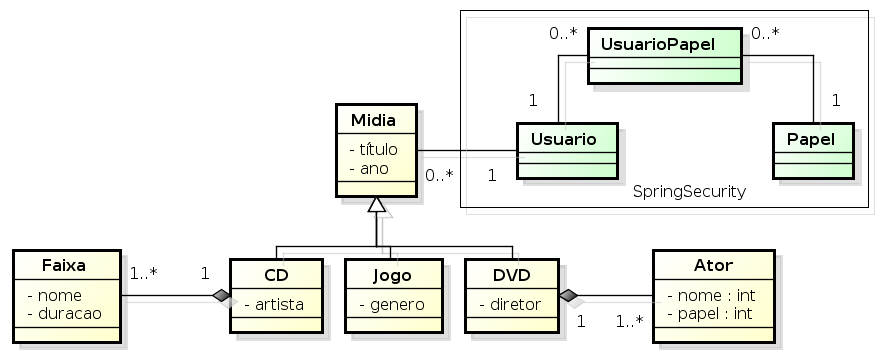
\includegraphics[width=14cm]{Midia}
\caption{Catálogo de Mídias.}
\label{MidiaFig}
\end{figure}

\subsection*{\underline{Entidade {\bf Midia}}}

A entidade  {\bf Midia} é uma  classe abstrata que deverá  conter atributos para
armazenar  os seguintes  dados  sobre as  mídias:  {\bf título}  e  {\bf ano  de
  criação}.

\subsection*{\underline{Entidade {\bf CD}}}

A entidade {\bf CD} (subclasse de {\bf Midia}) é uma classe que representa um CD
de  música e  deve  conter atributos  para  armazenar os  seguintes dados:  {\bf
  artista} (compositor/interpréte da  obra) e {\bf a lista  de faixas} (entidade
{\bf Faixa}). Vale a pena salientar que é um relacionamento {\bf 1 para N} entre
{\bf CD} e {\bf Faixa}.

\subsection*{\underline{Entidade {\bf Faixa}}}

A entidade {\bf  Faixa} é uma classe  que representa uma faixa de  música e deve
conter os seguintes  atributos: {\bf nome} da faixa e {\bf  duração} da faixa em
segundos.

\subsection*{\underline{Classe {\bf Jogo}}}

A classe {\bf  Jogo} (subclasse de {\bf Midia}) representa  um jogo eletrônico e
deve  conter o  seguinte atributo:  {\bf gênero}  do jogo  eletrônico (Esportes,
Corrida, RPG, Aventura, Tabuleiro, etc).

\subsection*{\underline{Entidade {\bf DVD}}}

A entidade {\bf  DVD} (subclasse de {\bf Midia}) é uma  classe que representa um
filme em  DVD e deve  conter atributos para  armazenar os seguintes  dados: {\bf
  diretor} do filme  e uma {\bf lista dos  principais atores/artistas} (entidade
{\bf Ator}) que atuaram no filme e  o papel desempenhado no filme.  Vale a pena
salientar que é um relacionamento {\bf 1 para N} entre {\bf DVD} e {\bf Ator}.

\subsection*{\underline{Entidade {\bf Ator}}}

A entidade  {\bf Ator} é uma classe  que representa um ator/atriz  e deve conter
atributos para armazenar os seguintes dados: o {\bf nome} do ator/atriz e o {\bf
  papel} desempenhado no filme .  

\subsection*{\underline{Entidades {\bf Usuario}, {\bf Papel} e {\bf UsuarioPapel}}}

A entidade {\bf Usuario} é uma classe que representa os usuário do sistema. Cada
usuário terá uma coleção de mídias (entidade {\bf Midia}) associadas a ele. Vale
a pena salientar  que é um relacionamento  {\bf 1 para N} entre  {\bf Usuario} e
{\bf Midia}  (As mídias  são categorizados em:  CDs de  música, filmes em  DVD e
jogos). 

\hspace{1cm}\\
\noindent A  entidade {\bf Papel} é uma  classe que representa os  papéis que os
usuários podem desempenhar.  Cada papel possui  permissões a ele associadas.  

\hspace{1cm}\\
\noindent  A  entidade  {\bf  UsuarioPapel}   é  uma  classe  que  representa  o
relacionamento muitos-para-muitos  entre usuários e papéis. Ou  seja, um usuário
pode  desempenhar vários  papeis e  um papel  pode ser  desempenhado  por vários
usuários.  

\hspace{1cm}\\
\noindent As entidades {\bf Usuario}, {\bf Papel} e {\bf UsuarioPapel} devem ser
geradas  através do  comando  {\bf  s2-quickstart} discutido  no  capítulo 3  do
material.  

\newpage

\section*{Observações importantes}

\vspace{0.3cm}

\begin{itemize}

\item É necessário a utilização do {\bf mecanismo de herança} e associações {\bf
  1 para N} para a implementação do catálogo.

\vspace{0.2cm}

\item Internacionalização (I18n)

\vspace{0.2cm}

\begin{itemize}

\item Português e uma língua estrangeira (Inglês, Francês, Alemão, Japonês, etc)

\end{itemize}

\vspace{0.2cm}

\item Autenticação

\vspace{0.2cm}

\begin{itemize}

\item  Simples: login/senha  (armazenado em  banco  de dados)  da entidade  {\bf
  Usuario}.  

\end{itemize}

\vspace{0.2cm}

\item Versão {\it grails} (mínimo): 3.1.4

\end{itemize}

% \section*{Funcionalidade: apresentar detalhes}

% \vspace{0.3cm}

% É  necessária a implementação  da funcionalidade  {\bf apresentar  detalhes} das mídias levando em consideração o tipo da mídia. Essa funcionalidade precisa está associada a  funcionalidade de  listagem das mídias.  Ou seja, quando  o usuário selecionar uma mídia, os seus detalhes precisam ser apresentados. 

% \begin{enumerate}

% \vspace{0.2cm}

% \item Detalhes de um CD de música

% \hspace{1cm}\\
% \begin{tabular}{|l|}
% \hline Título: Bachianas Brasileiras No.2 \\

% Ano: 2004 \\

% Tipo: CD de música \\

% Artista: Orquestra de Câmara da Universidade de São Paulo \\

% Faixa 1: (Prelúdio) O Canto do Capadócio, duracão: 8:32 \\

% Faixa 2: (Ária) O Canto da Nossa Terra, duracao: 6:29 \\

% Faixa 3: (Dança) Lembranca do Sertão, duracão: 5:24 \\

% Faixa 4: (Tocata) O Trenzinho do Caipira, duracão: 4:44 \\

% \hline
% \end{tabular}
% \newline

% \vspace{0.2cm}
% \item Detalhes de um filme em DVD

% \hspace{1cm}\\
% \begin{tabular}{|l|}
% \hline Título: O Senhor dos Anéis - A Sociedade dos Anéis \\

% Ano: 2001 \\

% Tipo: Filme em DVD \\

% Diretor: Peter Jackson \\

% Artista 1: Elijah Wood, papel: Frodo Baggins \\

% Artista 2: Viggo Mortensen, papel: Aragorn \\

% Artista 3: Orlando Bloom, papel: Legolas Greenleaf \\

% Artista 4: Christopher Lee, papel: Saruman \\

% Artista 5: Ian McKellen, papel: Gandalf \\

% \hline
% \end{tabular}
% \newline

% \vspace{0.2cm}
% \item Detalhes de um jogo

% \hspace{1cm}\\
% \begin{tabular}{|l|}
% \hline Título: {\it Need For Speed - Underground II} \\

% Ano: 2005 \\

% Tipo: Jogo Eletrônico \\

% Gênero: Corrida \\ \hline
% \end{tabular}

% \end{enumerate}

% \newpage

\section*{Funcionalidade: redirecionamento}

\vspace{0.3cm}

Implemente  uma página  de {\it  login} que  autentica os  usuários e  realiza o
direcionamento dependente do papel do usuário: 

\vspace{0.3cm}

\begin{itemize}

\item  Se papel  do usuário  é  {\bf Administrador},  direcione para  a lista  de
  usuários.

\vspace{0.3cm}

\item Se papel do usuário é {\bf Comum}, direcione para a lista de CDs do usuário
  logado.

\end{itemize}

% \section*{Funcionalidade: lista de CDs (apenas para RAs pares)}

% \vspace{0.3cm}

% \begin{itemize}

% \item Implemente a funcionalidade (página {\it  web}) de busca de CDs: com ajuda no preenchimento (autocomplete em AJAX) do nome do CD.  
 
% \vspace{0.3cm}

% \item Implemente um serviço web que retorna a lista de CDs de um dado artista: o parâmetro de entrada do serviço web é o nome do artista.

% \end{itemize}

% \section*{Funcionalidade: lista de DVDs (apenas para RAs ímpares)}

% \vspace{0.3cm}

% \begin{itemize}

% \item Implemente a funcionalidade (página {\it web}) de busca de DVDs: com ajuda no preenchimento (autocomplete em AJAX) do nome do DVD.  
 
% \vspace{0.3cm}

% \item Implemente um serviço web que retorna  a lista de DVDs de um dado diretor: o parâmetro de entrada do serviço web é o nome do diretor.

% \end{itemize}

% \vspace{0.3cm}






